\documentclass[problem]{mcs}

\begin{pcomments}
  \pcomment{FP_tetris_recurrence_well_order_variant}
  \pcomment{F03.rec2 using induction, S17.mid1}
  \pcomment{Lisa Sukharev-Chuyan and ARM revised for midterm1 2/21/17}
\end{pcomments}

\pkeywords{
  recurrence
  tetris
  tiling
}

%%%%%%%%%%%%%%%%%%%%%%%%%%%%%%%%%%%%%%%%%%%%%%%%%%%%%%%%%%%%%%%%%%%%%
% Problem starts here
%%%%%%%%%%%%%%%%%%%%%%%%%%%%%%%%%%%%%%%%%%%%%%%%%%%%%%%%%%%%%%%%%%%%%

\begin{problem}
\emph{Mini-Tetris} is a game whose objective is to provide a complete
``tiling'' of a $2 \times n$ board using tiles of specified shapes.
In this problem we consider the following set of five tiles:
\iffalse
 shown in
Figure~\ref{5tiles}.
\fi

\medskip
\centerline{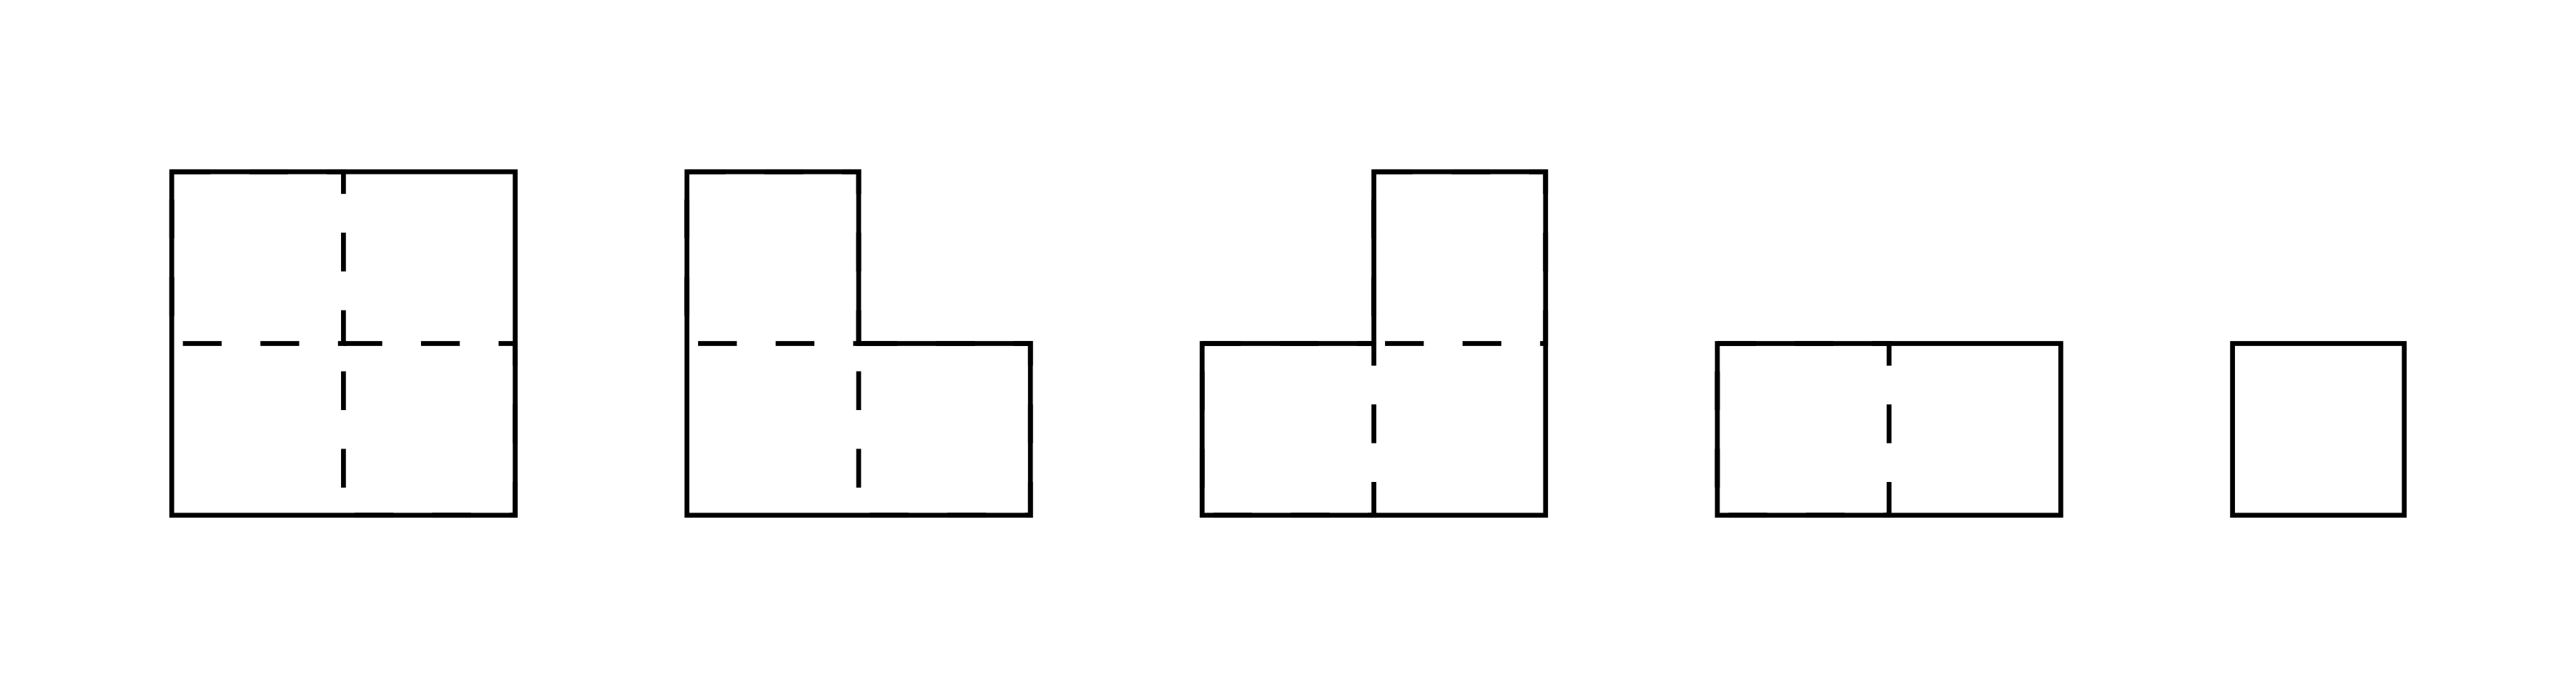
\includegraphics[height=1.25in]{tetris5pieces.png}}
\medskip

For example, there are two possible tilings of a $2 \times 1$ board:

\medskip
\centerline{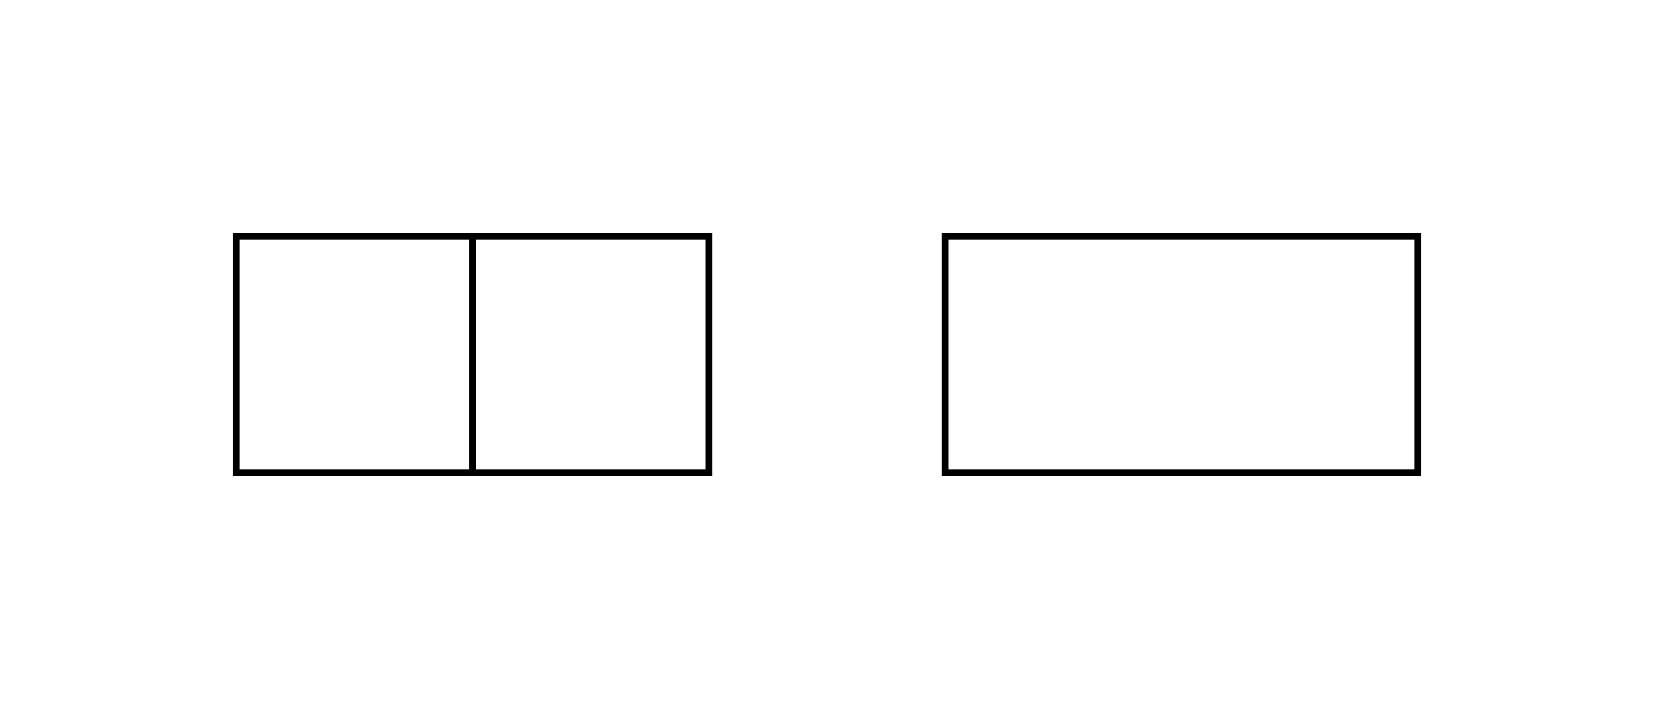
\includegraphics[height=1.25in]{tetris5pieces-1all.png}}
\medskip

Also, here are three tilings for a $2 \times 2$ board:

\medskip
\centerline{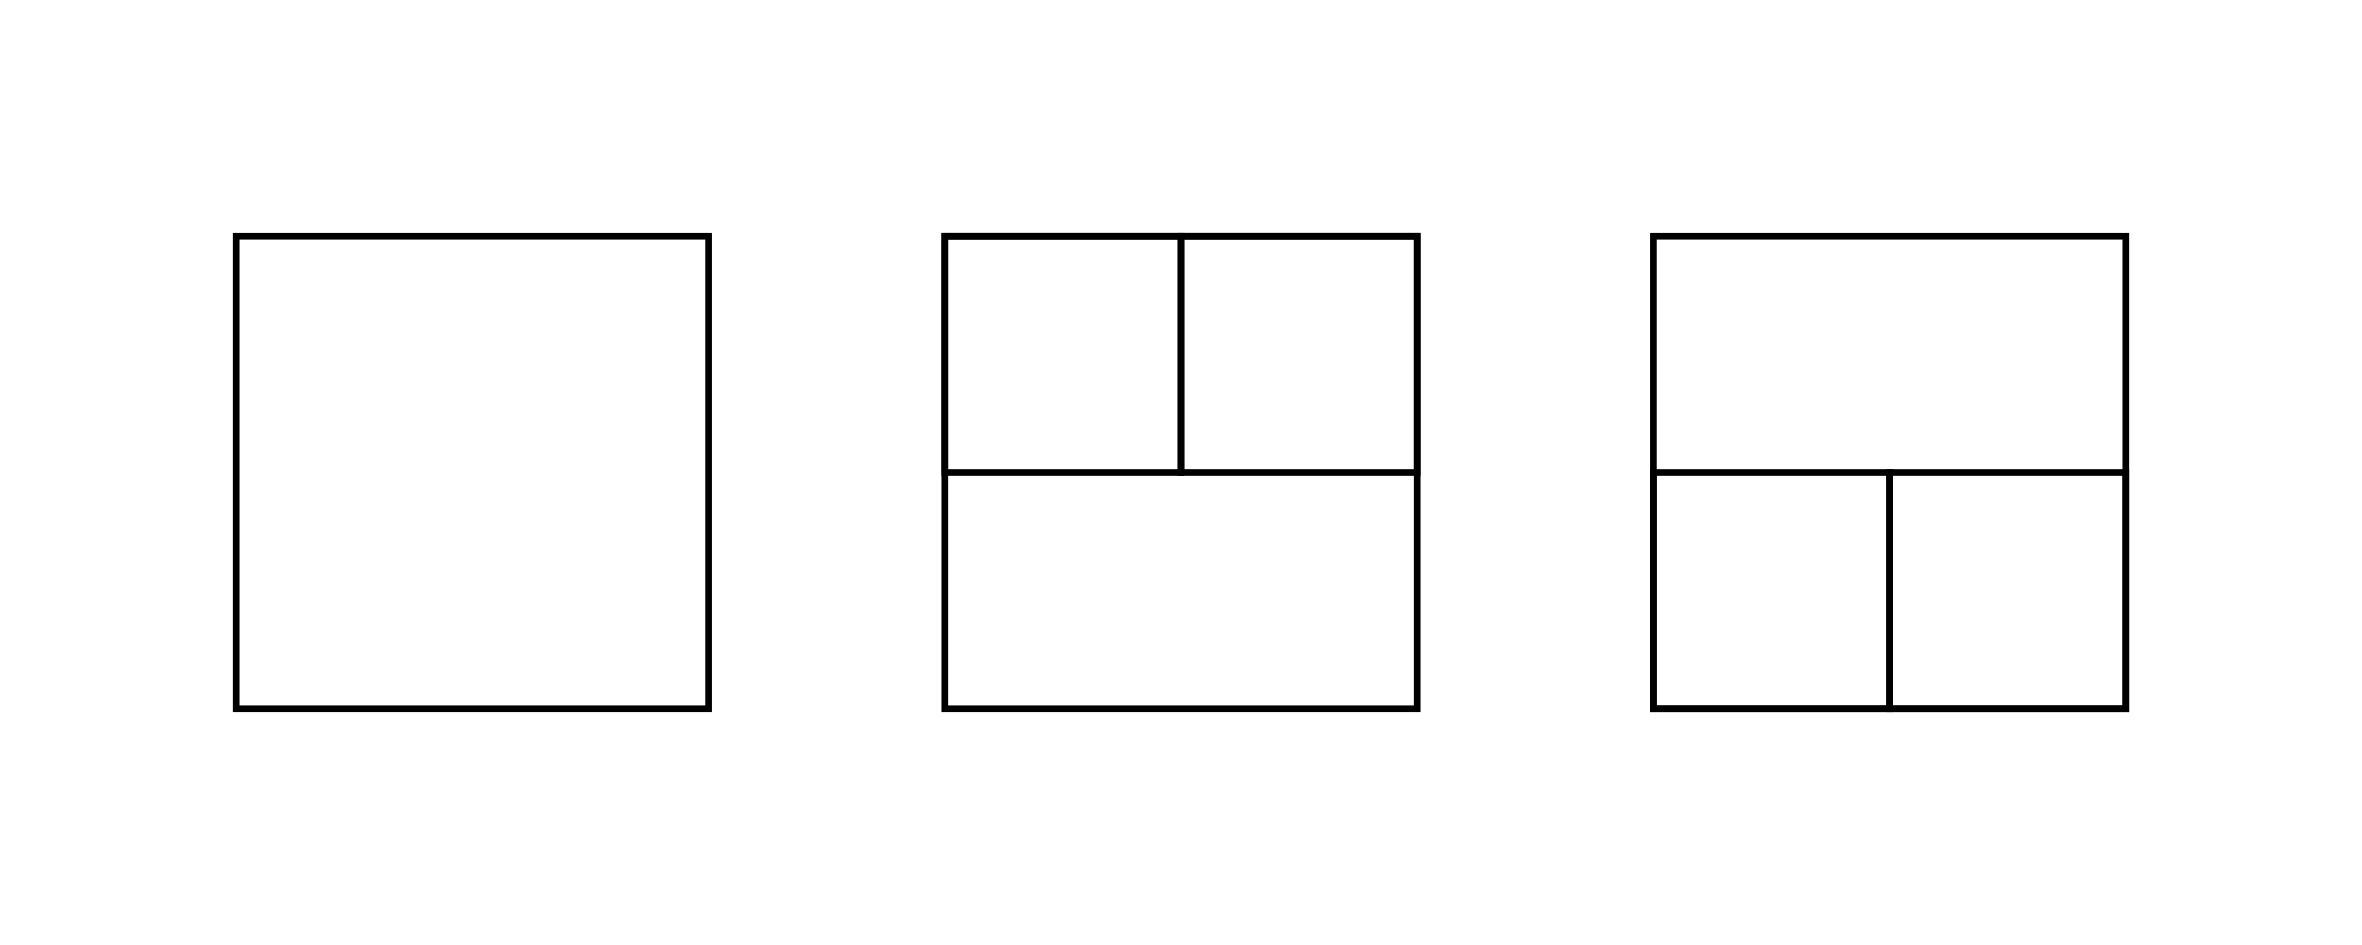
\includegraphics[height=1.25in]{tetris5pieces-2samples.png}}
\medskip

Note that tiles may not be rotated, which is why the second and third
of the above tilings count as different, even though one is a $180^o$
rotation of the other.  (A $90^o$ degree rotation of these shapes
would not count as a tiling at all.)

\begin{problemparts}

\problempart There are four more $2 \times 2$ tilings in addition to
the three above.  What are they?

\examspace[1.5in]

\begin{solution}

\medskip
\centerline{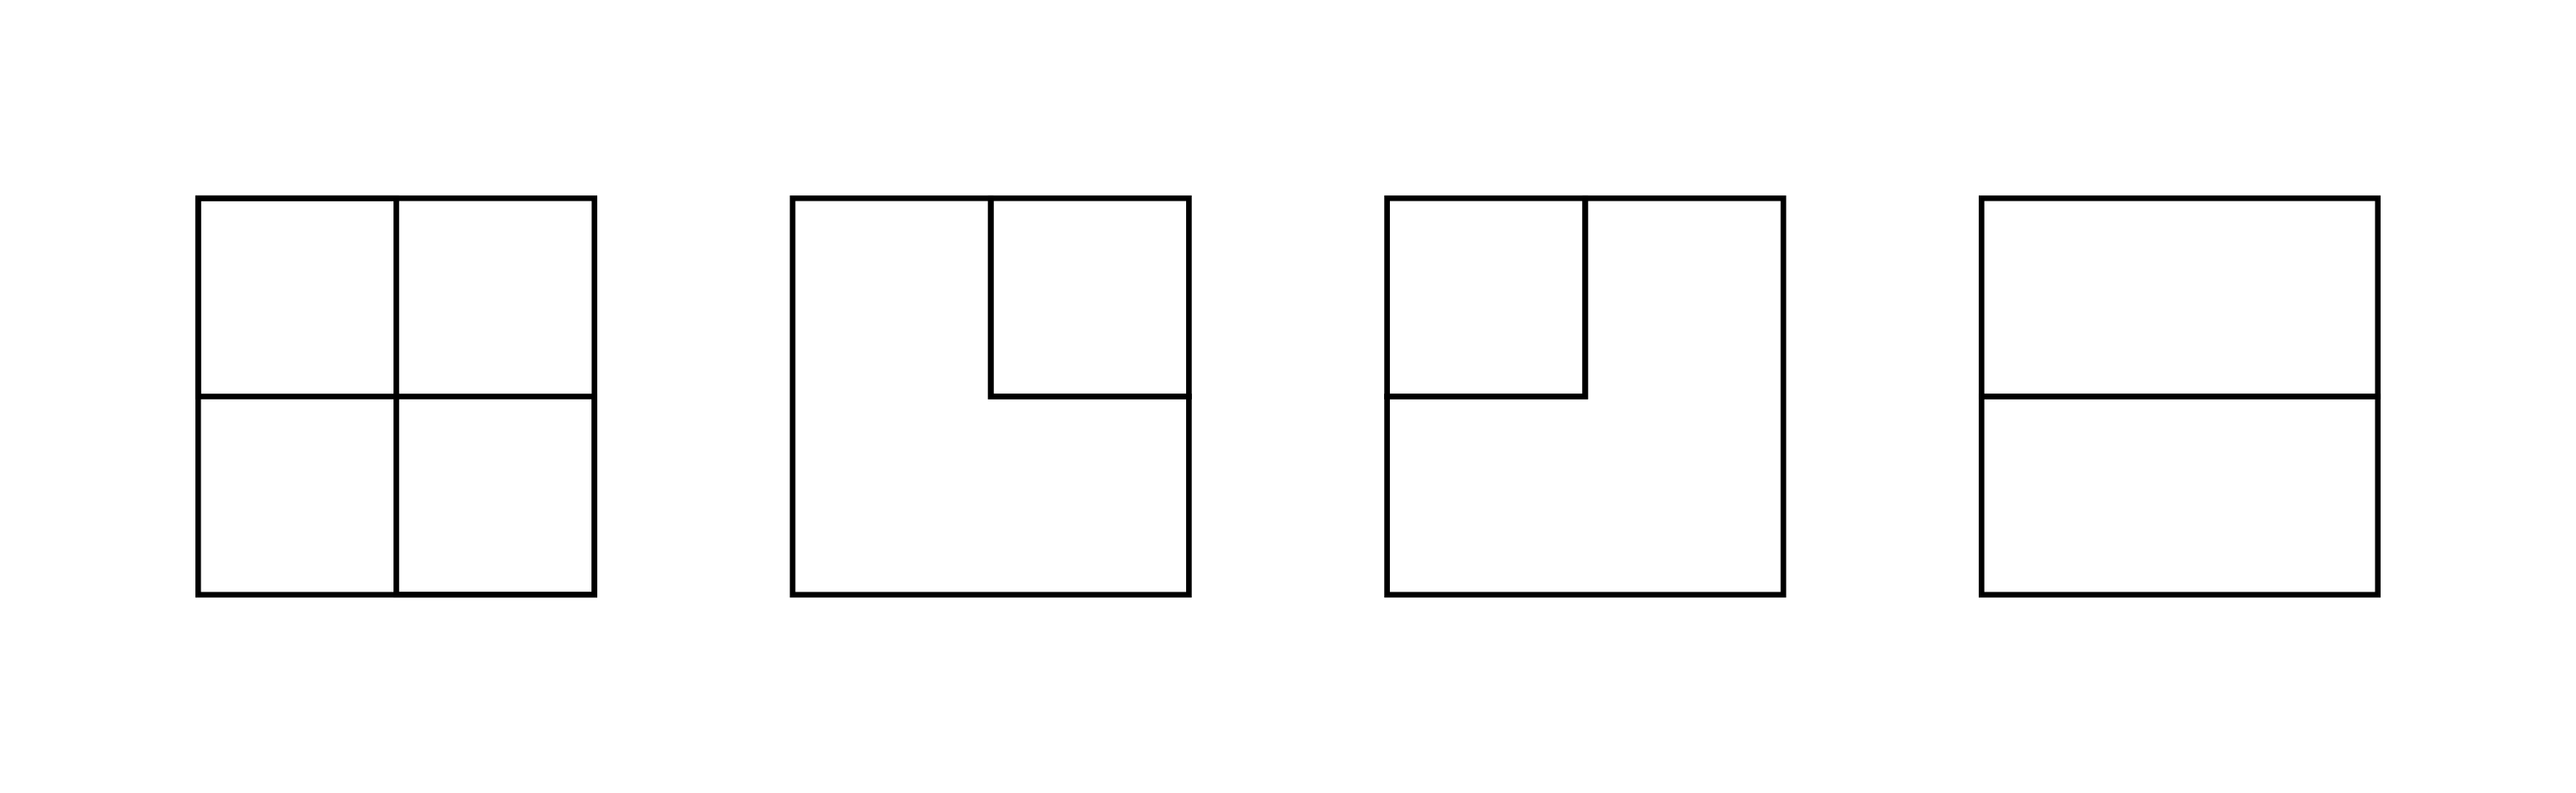
\includegraphics[height=1.25in]{tetris5pieces-2rest.png}}
\medskip

\end{solution}

\eparts

\examspace

Let $T_n$ denote the number of different tilings of a $2 \times n$
board.  We know that $T_1 = 2$ and $T_2 = 7$.  Also, $T_0=1$ because
there is exactly one way to tile a $2 \times 0$ board---don't use any
tiles.

\bparts

\problempart $T_n$ can be specified in terms of $T_{n-1}$ and
$T_{n-2}$ as follows:
\begin{equation}\label{tnn-1n-2}
T_n = 2T_{n-1} + 3T_{n-2}
\end{equation}
for $n\geq 2$.

Briefly explain how to justify this equation.

\examspace[2.5in]

\begin{solution}
Every winning tiling on a $2 \times n$ board is of one of the
following five types:

\medskip
\centerline{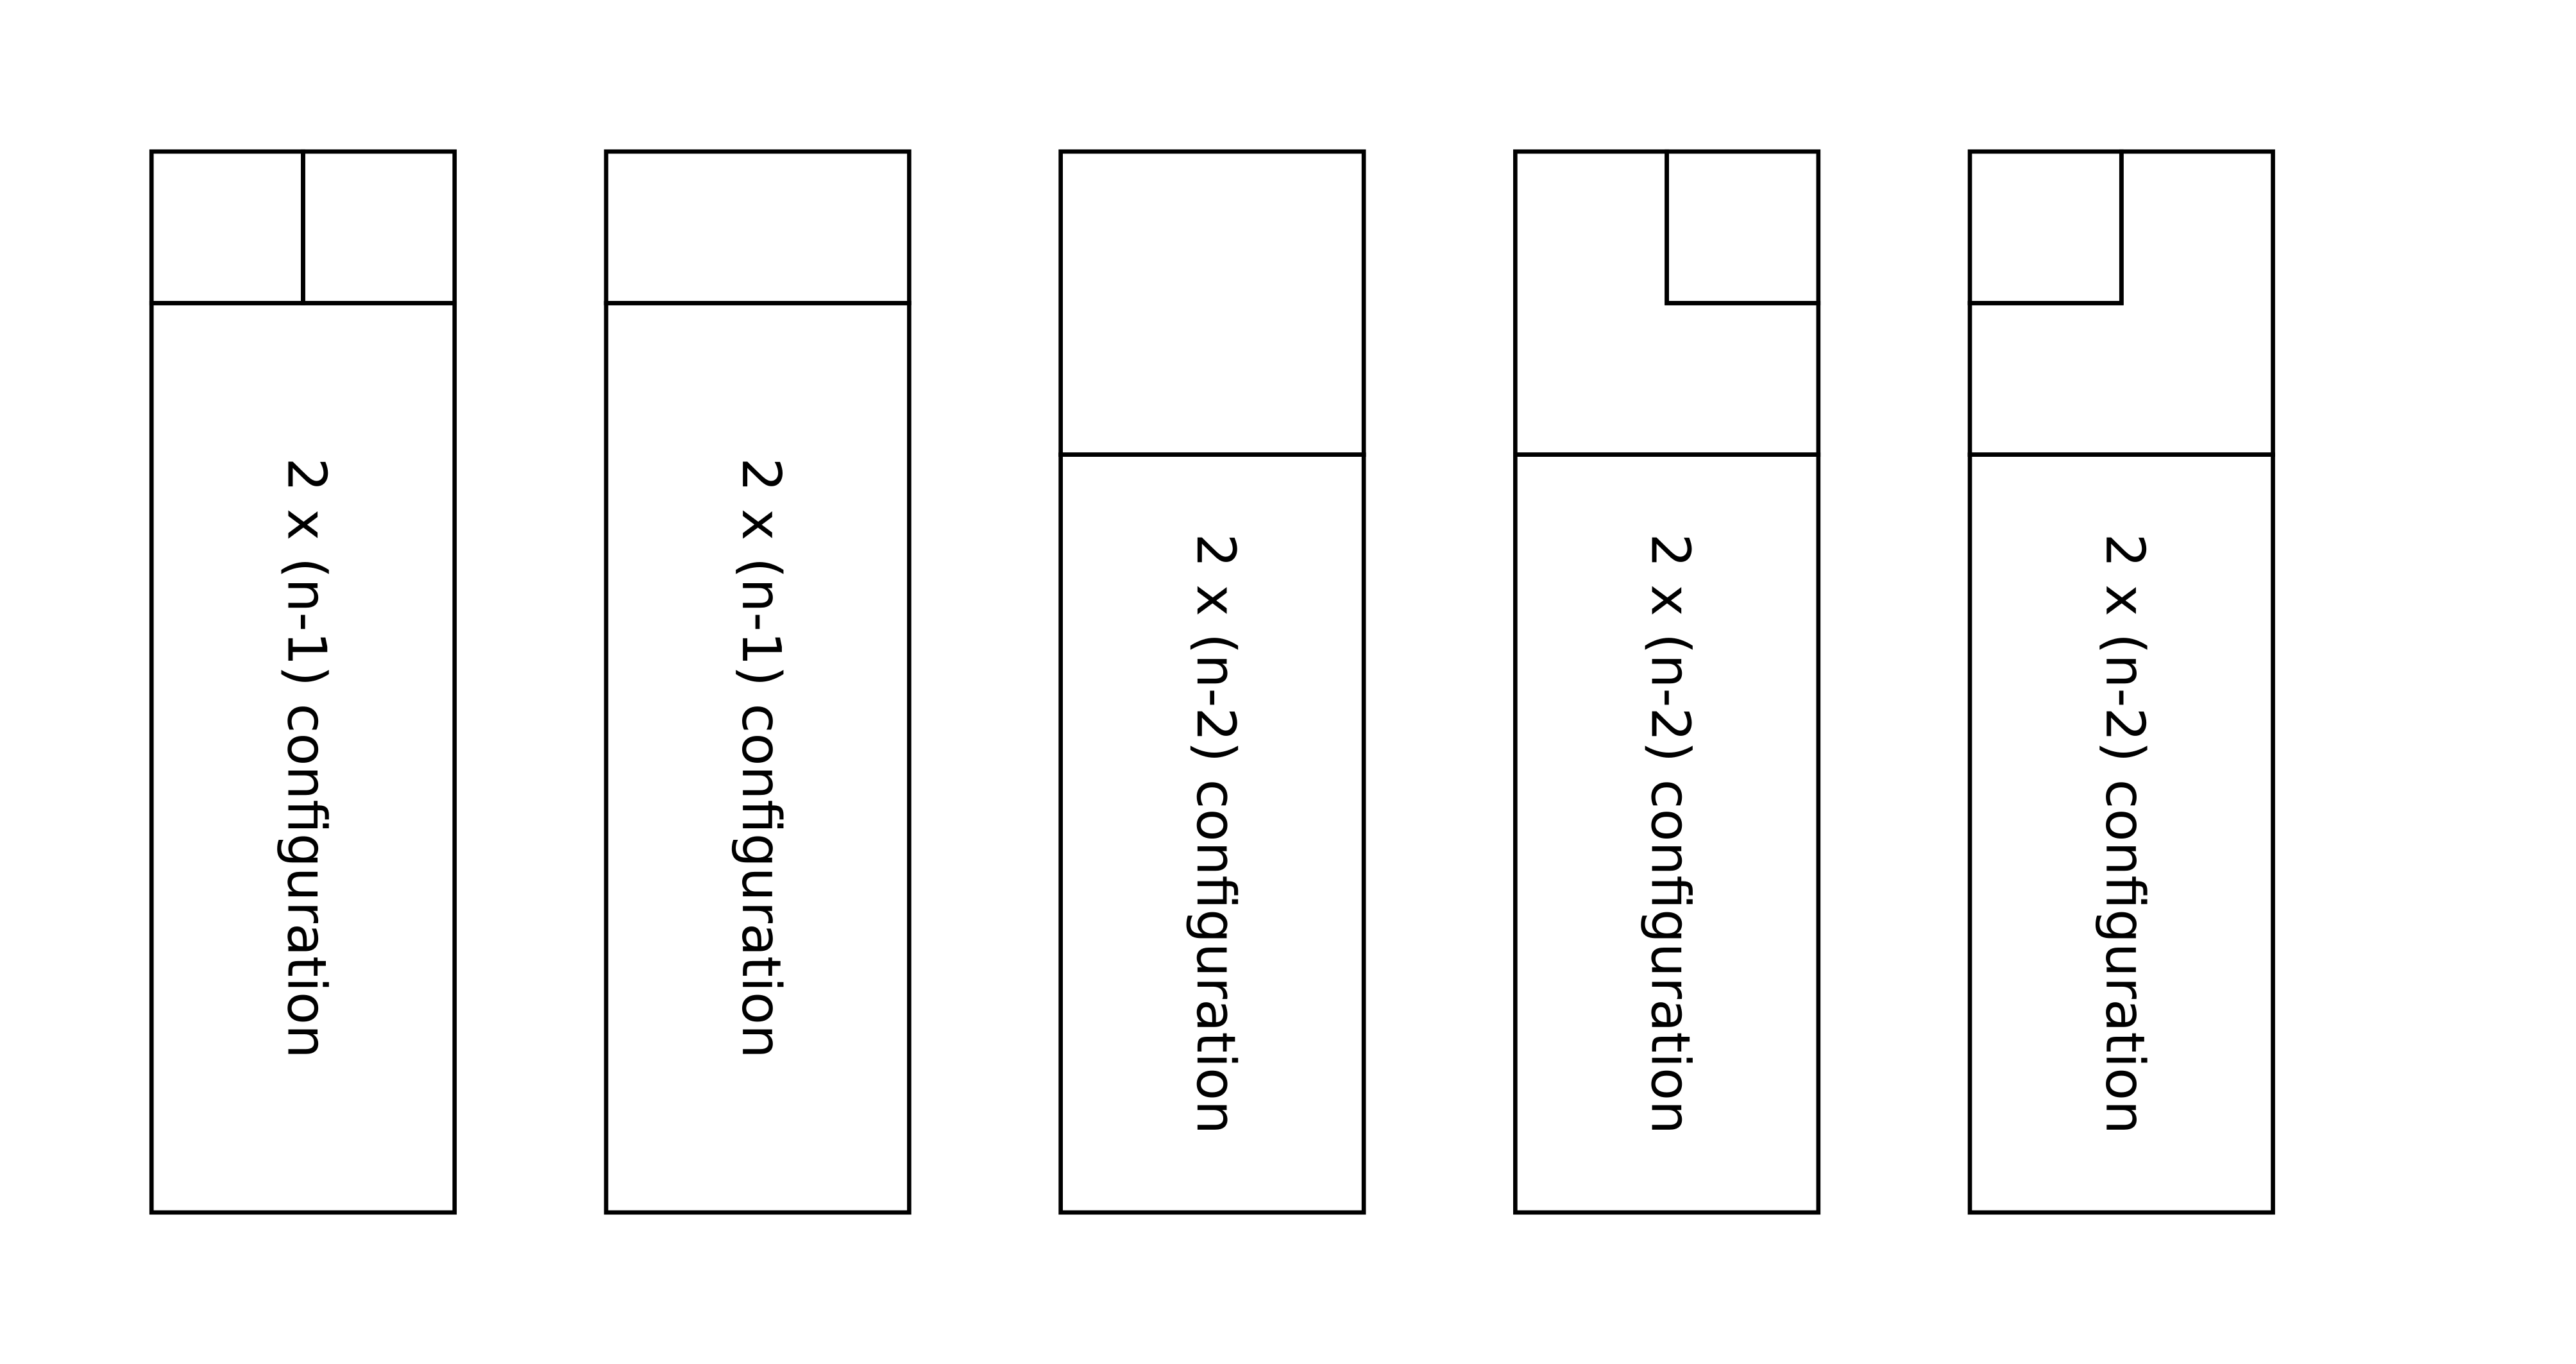
\includegraphics[height=1.25in]{tetris5pieces-kinds.png}}
\TBA{5tilingkinds}
\medskip

There are $T_{n-1}$ tilings for each of the first two types and
$T_{n-2}$ tilings for each of the last three types, so the total
number of $2 \times n$ tilings is given by the right hand side of
equation~\ref{tnn-1n-2}.
\end{solution}

\problempart Use the Well Ordering Principle to prove that for $n \geq
0$, the number $T_n$ of tilings of a $2 \times n$ Mini-Tetris board
is:
%\begin{equation}\label{3n+1-14}
\[
\frac{3^{n+1} + (-1)^n}{4}.
\]
%\end{equation}

\examspace[5.0in]

\begin{solution}
Let $P(n)$ be the predicate
\[
P(n) \eqdef\ \brac{T_n = \frac{3^{n+1}+(-1)^n}{4}},
\]
and let $C$ be the set of counterexamples to $P$:
\[ 
C \eqdef \set{n \ge 0 \suchthat \QNOT(P(n))}.
\]

Assume for the sake of contradiction that $C$ is not empty.  Then by
the Well Ordering Principle, there is some minimum element $m \in C$.
But $P(n)$ is true for $n=0,1$:
\begin{align*}
T_0 & = 1 = \frac{3^{(0+1)}+(-1)^0}{4}, \\
T_1 & = 2 = \frac{3^{(1+1)}+(-1)^1}{4}.
\end{align*}
This means that $m$ must be greater than 1.  So both $m-1$ and $m-2$
are $\geq 0$, and since $m$ is the smallest nonnegative
counterexample, neither $m-1$ nor $m-2$ is a counterexample.  That is,
$P(m-1)$ and $P(m-2)$ are true.

Thus, we have
\begin{align*}
T_m & = 2 T_{m-1}+3T_{m-2} 
          & \text{(by~\eqref{tnn-1n-2})}\\
    & =	2\frac{3^{m}+(-1)^{m-1}}{4} + 3\frac{3^{m-1}+(-1)^{m-2}}{4}
          & \text{(by $P(m-1)$ and $P(m-2)$)}\\
    & = \frac{2(3^{m}+(-1)^{m-1})+3(3^{m-1}+(-1)^{m-2})}{4}\\
    & = \frac{2(3^{m})+ 3^m + (-2+3)(-1)^{m}}{4}\\
    & = \frac{3^{m+1}+(-1)^{m}}{4}.
\end{align*}
This shows that $P(m)$ is true, contradicting the definition of $m$.
So $C$ must be empty, which proves that $P(n)$ is true for all $n\geq
0$, as desired.
\end{solution}

\end{problemparts}

\end{problem}

\endinput
